\documentclass[../../main.tex]{subfiles}
\begin{document}
\chapter{Multi-Track and Non-Linear Synthesis}
\label{ch:multi_track}

Human movement is a symphony of coordinated actions, where each part of the body plays a distinct role, yet all work together in harmony to create a seamless expression of intent. The essence of this coordination lies in the ability to perform multiple actions simultaneously or in carefully timed sequences, with each movement contributing to the larger tapestry of physical expression. Traditional approaches to understanding or replicating this complexity often fall short, reducing human motion to a linear series of bone rotations that lack the depth and nuance of true human movement.

The concept of multi-track control offers a different perspective—one that acknowledges the layered nature of our physical existence. It recognizes that our movements are not isolated but interwoven, with each gesture or posture influencing and being influenced by others. By allowing multiple threads of action to unfold concurrently or in precise intervals, multi-track control mirrors the natural rhythm and flow of life. It captures the interplay between stillness and motion, the balance of tension and release, and the silent dialogue between different parts of the body as they move together yet independently. In doing so, it brings us closer to understanding the profound complexity of human movement, honoring the subtlety and grace inherent in every action.

Similarly, non-linearity in movement reflects the dynamic and adaptive nature of human actions. Just as life rarely follows a straightforward path, our movements often involve layers of simultaneous actions that interact in complex ways. In fields like video editing or film production, non-linear control allows creators to work with multiple layers of footage, sounds, and effects, enabling them to craft scenes where various elements unfold together, contributing to a richer and more cohesive narrative.

In the realm of sign language, the non-linear and multi-track nature of human movement is particularly evident. Sign language involves a combination of simultaneous gestures, facial expressions, and body movements, all working together to convey meaning. By adopting a non-linear, multi-track approach, we can more accurately capture the intricate coordination involved in signing, where gestures and expressions occur in parallel, influencing and overlapping with each other. This approach respects the complexity and interconnectivity inherent in sign language, allowing for a more nuanced and realistic portrayal of its dynamic and expressive nature. In doing so, it brings us closer to truly understanding and representing the fluidity and richness of sign language as it is naturally used, honoring its depth and complexity as a form of human communication.

This chapter aims to present a novel approach to sign language synthesis using multi-track and non-linear editing techniques. It showcases improvements in animation quality and flexibility, demonstrating how these techniques preserve the dynamics of individual animation blocks and enhance procedural generation capabilities.

The content of this chapter is structured as follows: Section~\ref{ch:multi_track:related_work} provides an overview of related work in the field of multi-track and non-linear editing, highlighting existing approaches and their applications. Section~\ref{ch:multi_track:score_to_timeline} introduces the concept of converting an AZee Synced Score into a multi-track timeline, outlining the process and benefits of this approach. Section~\ref{ch:multi_track:azee_nl} explores the implications of non-linear synthesis in AZee, discussing how the order of block evaluation can affect the final animation. Section~\ref{ch:multi_track:resolve_conflitcs} addresses the issue of resolving conflicts between blocks in the multi-track timeline, presenting rules and strategies for ensuring smooth and accurate animation. Section~\ref{ch:multi_track:second_pass} describes the second pass evaluation process, focusing on cyclic block sets, transpath blocks, and hold blocks. Section~\ref{ch:multi_track:preanim_blocks} discusses the integration of pre-animated blocks into the multi-track timeline, highlighting the benefits and challenges of this approach. Finally, Section~\ref{ch:multi_track:implem_results} presents the implementation details and results of the multi-track and non-linear synthesis approach, showcasing the improvements in animation quality and flexibility achieved through this method.

\section{Related Work}
\label{ch:multi_track:related_work}

Both multi-track and non-linear editing have been widely used in various fields, including film production, video editing(figure~\ref{fig:video_edit}), and animation (figure~\ref{fig:nle_blender}). 

\begin{figure}[h]
    \centering
    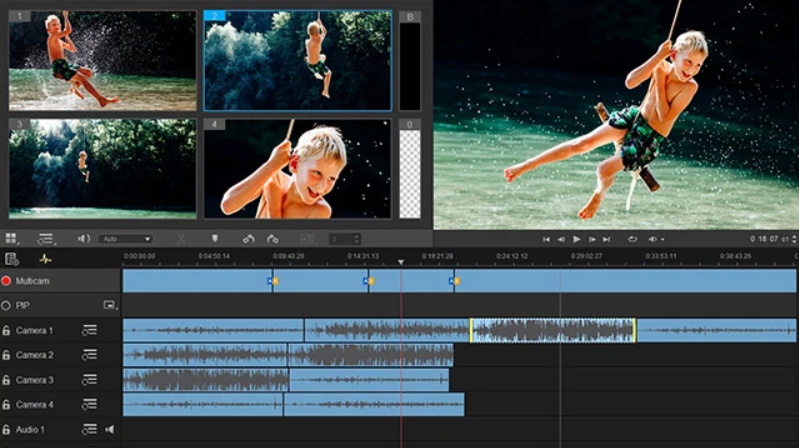
\includegraphics[width=0.8\textwidth]{chapters/multi_track/images/video_editing.png}
    \caption{Video editing software interfaces with multiple tracks for editing video and audio clips.}
    \label{fig:video_edit}
\end{figure}

\begin{figure}[h]
    \centering
    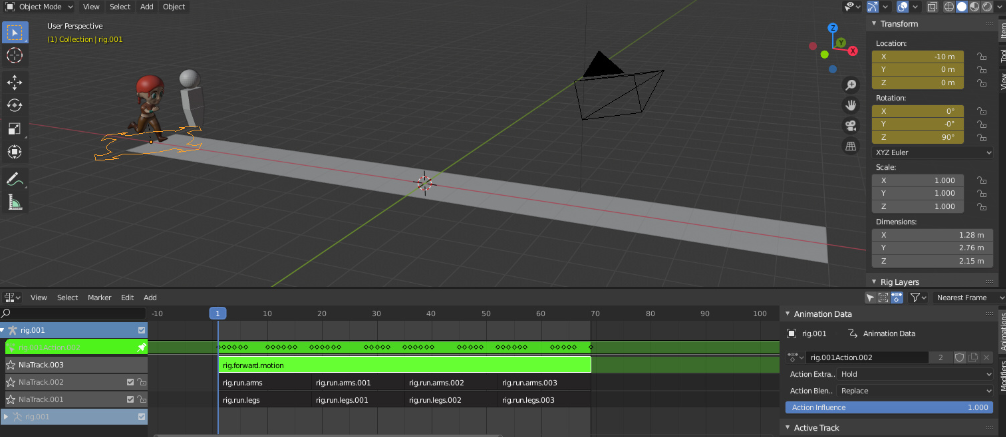
\includegraphics[width=0.8\textwidth]{chapters/multi_track/images/nle_blender.png}
    \caption{Blender's non-linear editor interface showing multiple tracks for editing animation clips.}
    \label{fig:nle_blender}
\end{figure}

However, their appliations in both procedural animation and sign language synthesis are limited.

\subsection{Existing low-level AZee synthesizor}
\label{ch:multi_track:related_work:old_azee_synthesizor}

Although AZee is multi-track by nature (where the lingusit has the ability to crate the track), the low-level AZee synthesizor is based on a flattened \emph{AnimatedScore} representation that flattenes each track made by the linguist. This flattening layer loses the multi-track information and the dynamics of the original AZee description. 

For example, consider the following low-level AZee description for \emph{:cupboard} when compiled with the AZee interpreter generates an AZee \emph{SyncedScore} using the algorithm~\ref{alg:azee_recursion}~\cite{filhol2017synthesizing} that is show in in figure~\ref{fig:azee_synced_score}.

\begin{figure}[h]
    \centering
    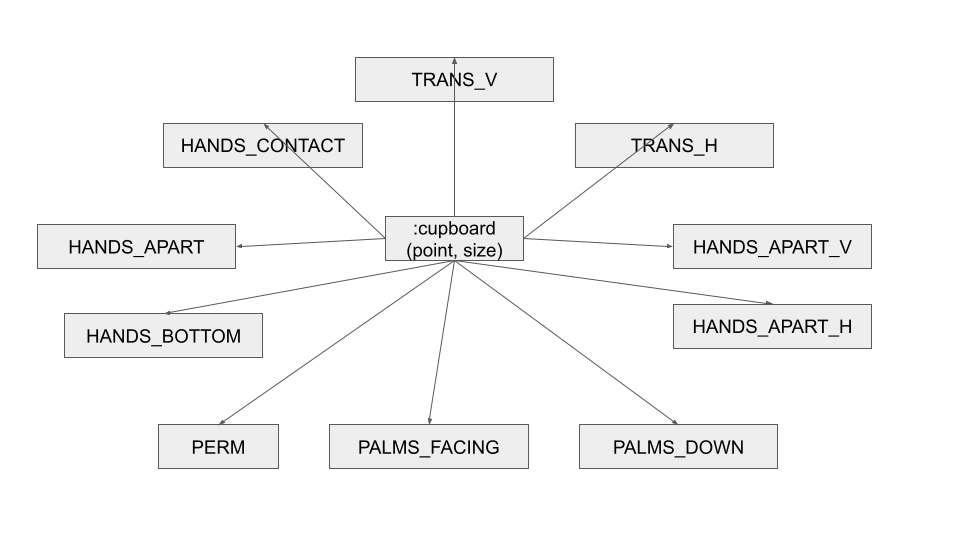
\includegraphics[width=0.8\textwidth]{chapters/multi_track/images/azee_synced_score.png}
    \caption{AZee Synced Score generated from the low-level AZee description.}
    \label{fig:azee_synced_score}
\end{figure}

Figure~\ref{fig:azee_flattened_score} shows the flattened version of this AZee Synced Score, where all the tracks are merged into a single track. This flattening is done by collecting all the constraints for each frame and applying them to the corresponding bone rotations during animation.

\begin{figure}[h]
    \centering
    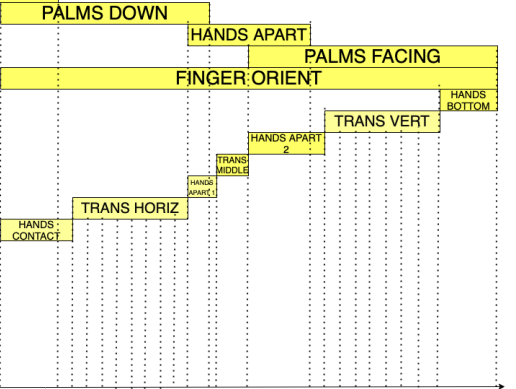
\includegraphics[width=0.8\textwidth]{chapters/multi_track/images/azee_flattened_score.png}
    \caption{Flattened version of the AZee Synced Score.}
    \label{fig:azee_flattened_score}
\end{figure}

This approach is also inextensible to be used with pre-animated motion data blocks for larger sequences since the flattened representation does not contain the original location of the corresponding animation block on the timeline. 

\subsection{Paula}
\label{ch:multi_track:related_work:paula}

On the contrary, a multi-track approach to sign language synthesis has already been done by~\cite{filhol2017synthesizing}. Paula is a multi-track sign language synthesis system that strictly uses pre-recorded motion data. The system is based on a multi-track timeline where each track is created by the artist(or can be based on the AZee description). The Paula interface is shown in figure~\ref{fig:paula}.

\begin{figure}[h]
    \centering
    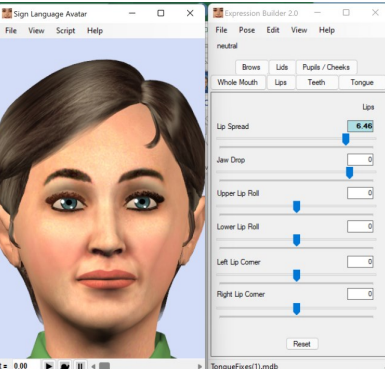
\includegraphics[width=0.8\textwidth]{chapters/multi_track/images/paula.png}
    \caption{Paula interface showing a multi-track timeline for sign language synthesis.}
    \label{fig:paula}
\end{figure}

However, Paula doesn't support low-level synthesis from AZee descriptions. This poses a challenge in scalability since an artist is always needed to create the building blocks of the animation. Although, the interface is tailored specifically for creating sign language content, a human intervention is still needed. Another drawback of Paula is that it is based on a single avatar model, which limits the diversity of the animations that can be created.

\subsection{Outside Sign Language Synthesis}
\label{ch:multi_track:related_work:other_multi_track}

The concept of multi-track timeline control for text-driven 3D human motion generation was also explored by~\cite{petrovich24stmc}. The work introduces a novel way to address the limitations of previous methods that lacked fine-grained control over action composition and timing. This approach allows users to define multiple textual prompts within overlapping temporal intervals, enabling precise control over complex actions (figure~\ref{fig:multi_track_other}). The proposed Spatio-Temporal Motion Collage (STMC) method, which operates at test-time, integrates with pre-trained motion diffusion models to generate realistic motions that adhere to the specified timeline. However, it is not for use in sign language synthesis, where precise and context-sensitive hand and body gestures are required, as it relies heavily on models not specifically designed for such detailed tasks.

\begin{figure}
    \centering
    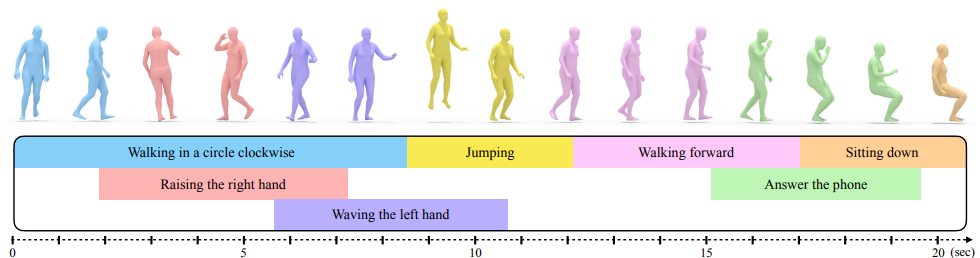
\includegraphics[width=0.8\textwidth]{chapters/multi_track/images/multi_track_other.png}
    \caption{Multi-track timeline control for text-driven 3D human motion generation.}
    \label{fig:multi_track_other}
\end{figure}

\section{AZee Synced Score to Multi-Track Timeline}
\label{ch:multi_track:score_to_timeline}

One of the areas which this work aims to address is the direct creation of a multi-track animation timeline from a multi-track AZee Synced Score. This approach allows for the preservation of the original multi-track information and dynamics present in the AZee description. The algorithm~\ref{alg:azee_timeline} shows how the AZee Synced Score is converted into a multi-track timeline.

\begin{algorithm}
    \caption{AZee Recursion Algorithm (Simplified)}
    \label{alg:azee_timeline}
    \begin{algorithmic}[1]
        \Function{CreateBlocks}{name, score, parent\_name, parent\_score, dynamic\_points}
            \If {parent\_score is not None}
                \State name $\gets$ name + "." + parent\_name
                \State \Call{UpdateSyncRules}{parent\_score, name}
            \EndIf
            
            \State \Call{UpdateBlockTimings}{name, score, parent\_name, parent\_score}
            \If {score.dynamic\_point}
                \State dynamic\_points.append(score.dynamic\_point)
            \EndIf
            
            \If {shortcut\_action $\gets$ \Call{GetShortcutAction}{score} \textbf{and} UseShortcutActions()}
                \State \Return \Call{CreateShortcutBlock}{name, score, parent\_score}
            \ElsIf {score is a SyncedScore}
                \For {child\_name, child\_score in score.block\_contents}
                    \State \Call{CreateBlocks}{child\_name, child\_score, name, score, dynamic\_points}
                \EndFor
            \Else
                \State \Return \Call{CreateRegularBlock}{name, score, parent\_score}
            \EndIf
            
            \If {parent\_score is not None}
                \State \Call{UpdateParentTimings}{parent\_name, name}
            \EndIf
        \EndFunction
    \end{algorithmic}
\end{algorithm}

The figure~\ref{fig:azee_timeline} shows the multi-track timeline generation for \emph{:cupboard}.

\begin{figure}[h]
    \centering
    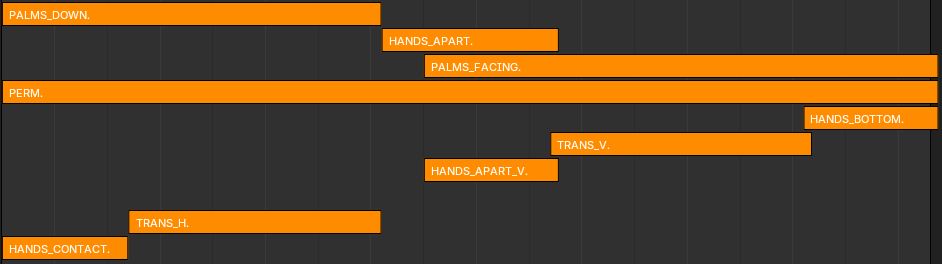
\includegraphics[width=0.8\textwidth]{chapters/multi_track/images/azee_timeline.png}
    \caption{Multi-track timeline generation from an AZee Synced Score.}
    \label{fig:azee_timeline}
\end{figure}

\section{AZee and Non-Linearity}
\label{ch:multi_track:azee_nl}

The order of synthesis of the blocks in the multi-track timeline is crucial for avoiding conflicts and ensuring the correct execution of constraints. Thus, an action which happens later in the timeline might be synthesized first. This makes the synthesis non-linear. Figure~\ref{fig:example_azee_non_linear} shows an example of non-linear synthesis.

\begin{figure}[h]
    \centering
    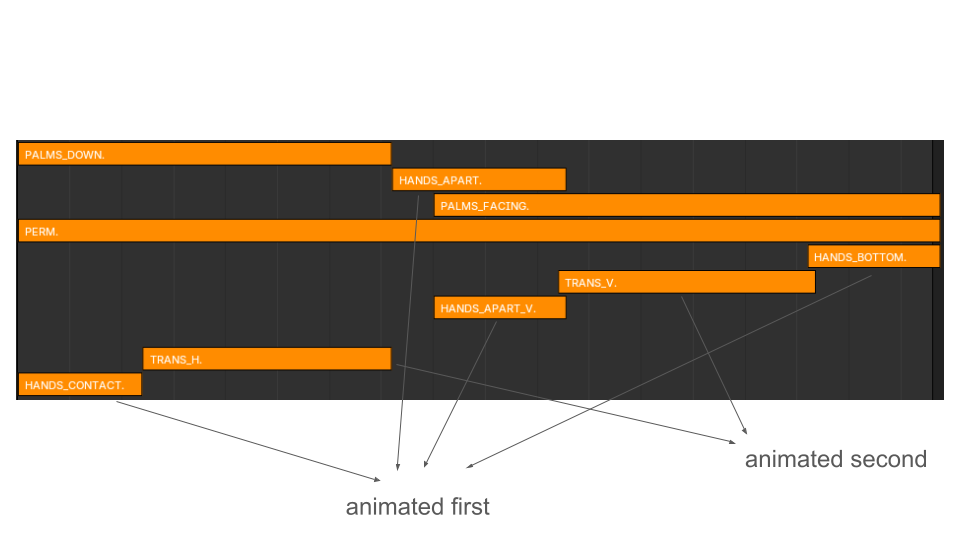
\includegraphics[width=0.8\textwidth]{chapters/multi_track/images/example_azee_non_linear.png}
    \caption{Example of non-linear synthesis in AZee.}
    \label{fig:example_azee_non_linear}
\end{figure}

\section{Resolving Block Conflicts}
\label{ch:multi_track:resolve_conflitcs}

Since the blocks in the multi-track timeline can have constraints that affect the same body parts, conflicts can arise. These conflicts need to be resolved to ensure the correct execution of the constraints. The following rules are used to resolve conflicts:

\subsection{ConstraintDAG}
\label{ch:multi_track:resolve_conflitcs:constraint_dag}

The constraints in the blocks can be represented as a Directed Acyclic Graph (DAG) where the nodes are the constraints and the edges represent the dependencies between the constraints. During evaluation, a topological sort enables that no linguistic constraint is broken. The figure~\ref{fig:constraint_dag_armoire} shows example of a ConstraintDAG for the block HANDS_CONTACT for the sign\emph{cupboard}. A more complex DAG of constraints can be seen in figure~\ref{fig:constraint_dag_tree} for the sign \emph{tree}.

\begin{figure}[h]
    \centering
    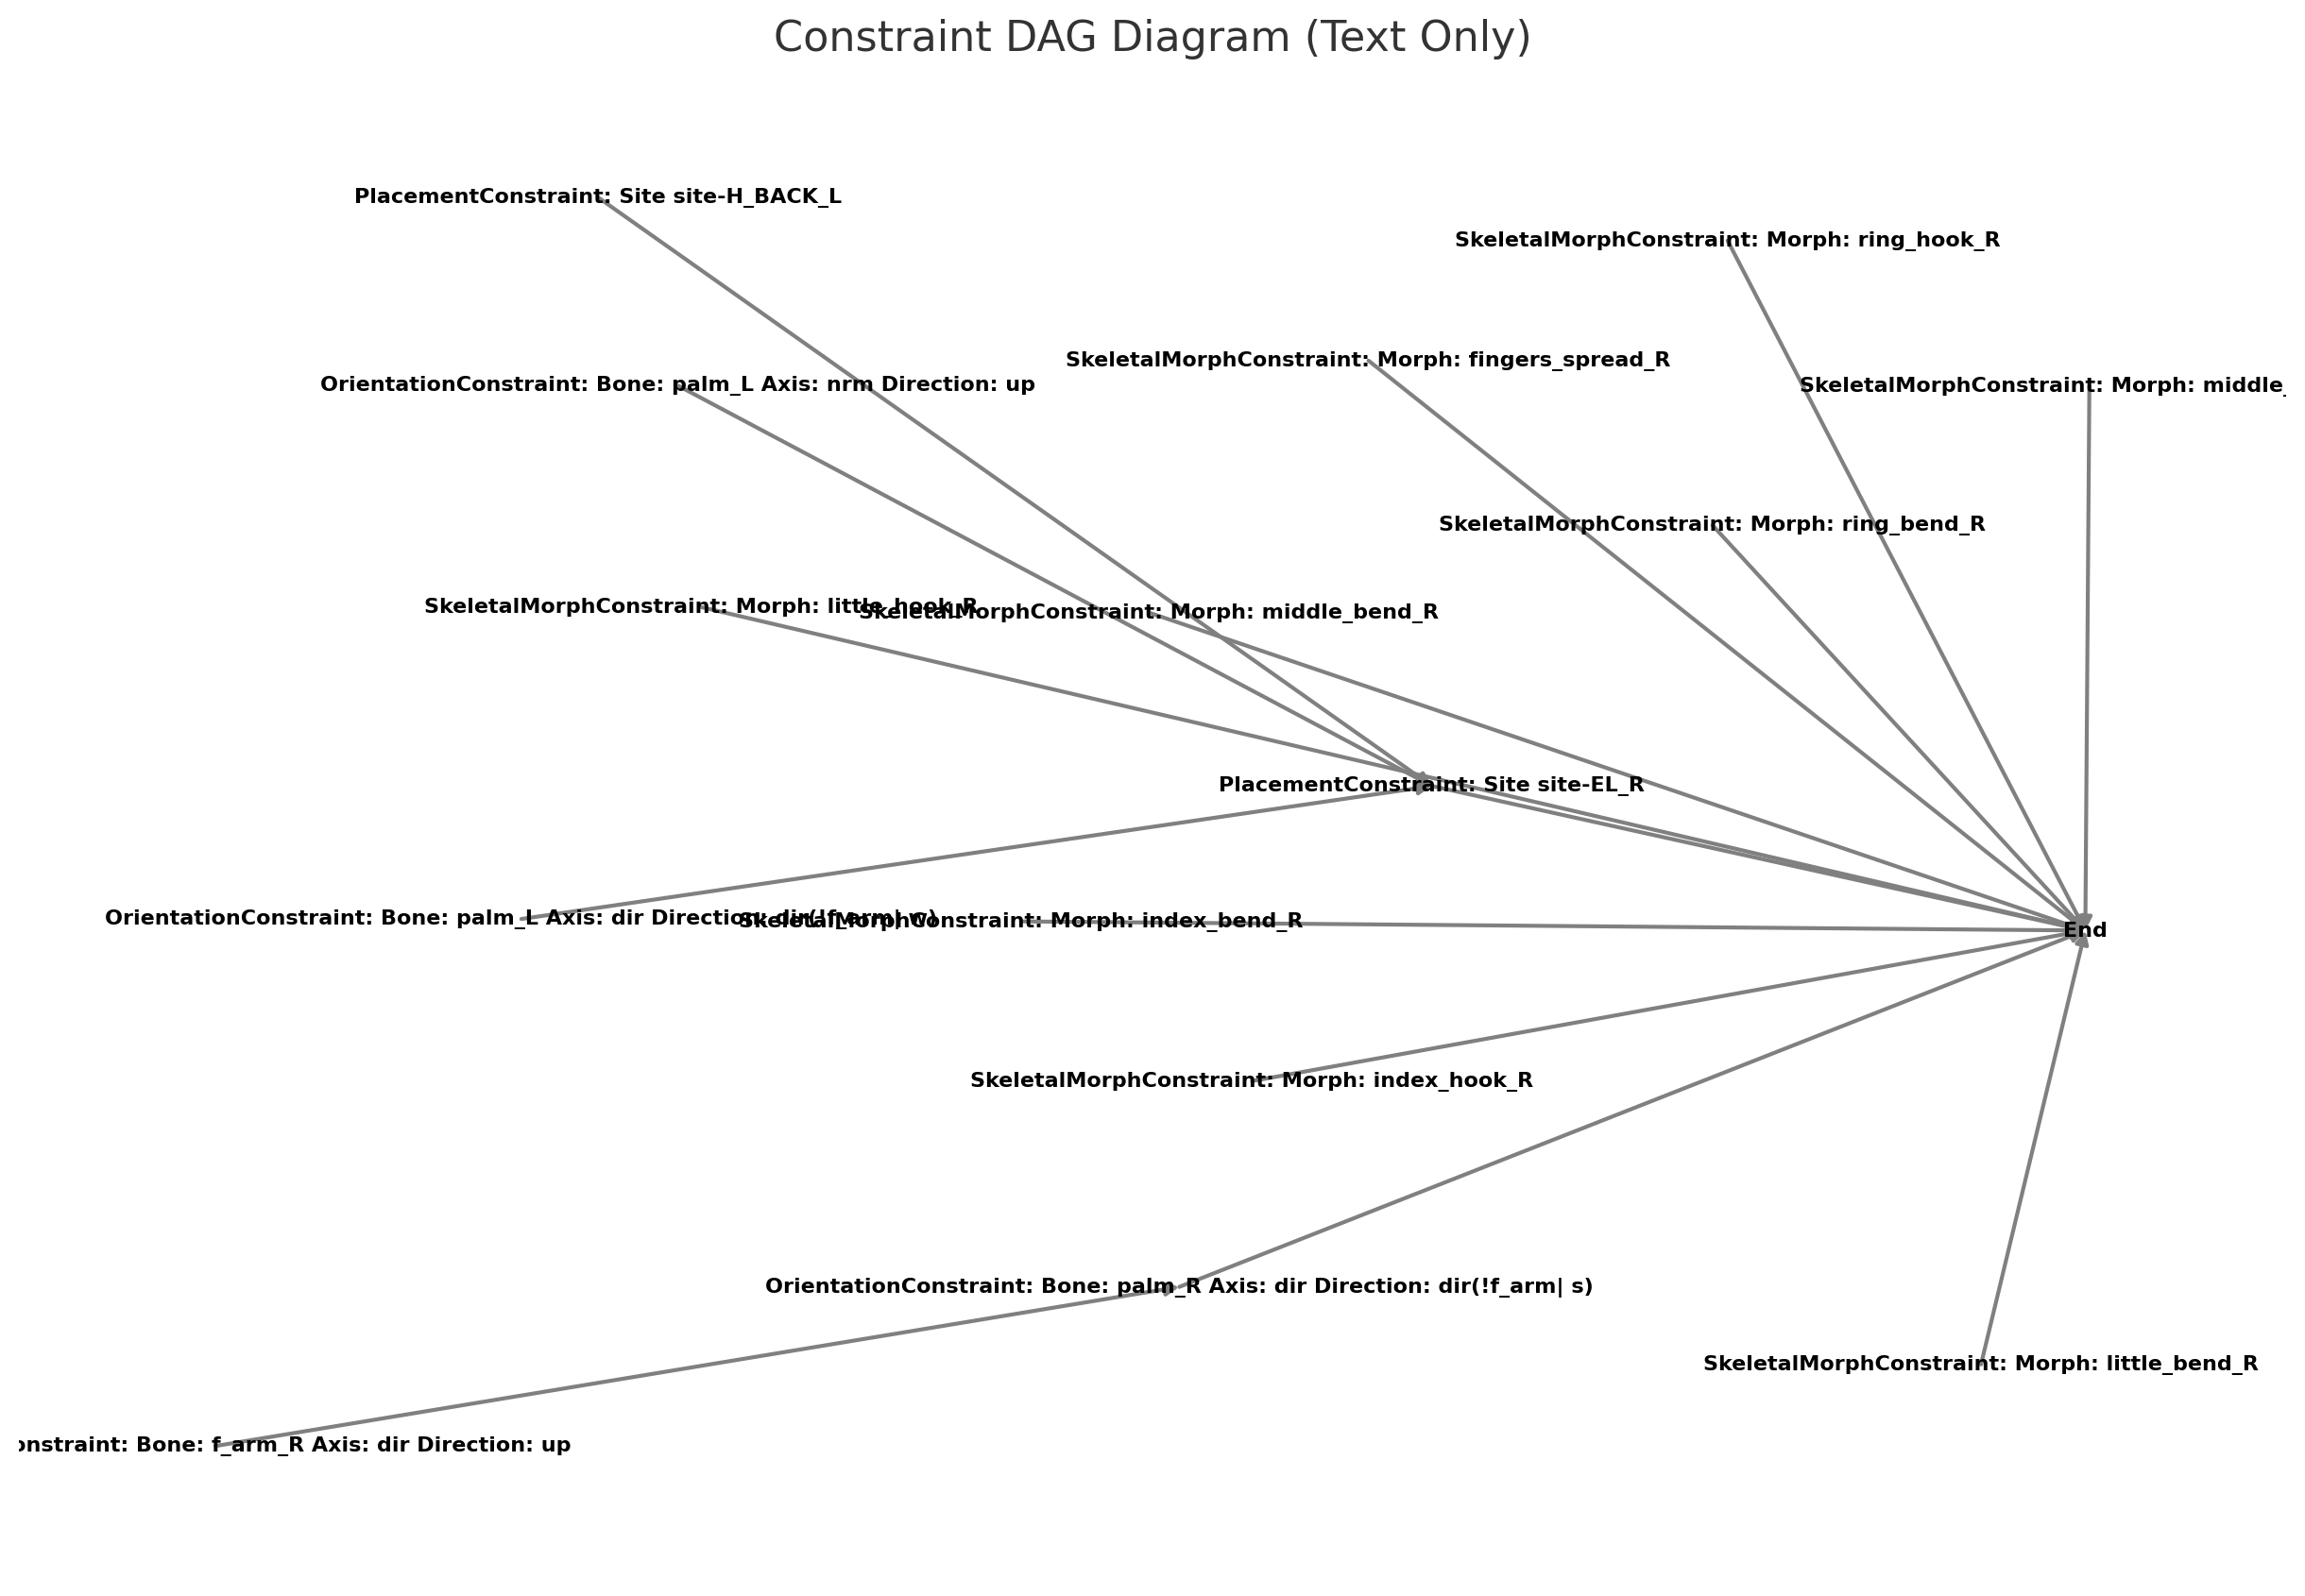
\includegraphics[width=0.8\textwidth]{chapters/multi_track/images/constraint_dag.png}
    \caption{ConstraintDAG for a single block discource for the sign \emph{tree}.}
    \label{fig:constraint_dag_tree}
\end{figure}

\begin{figure}[h]
    \centering
    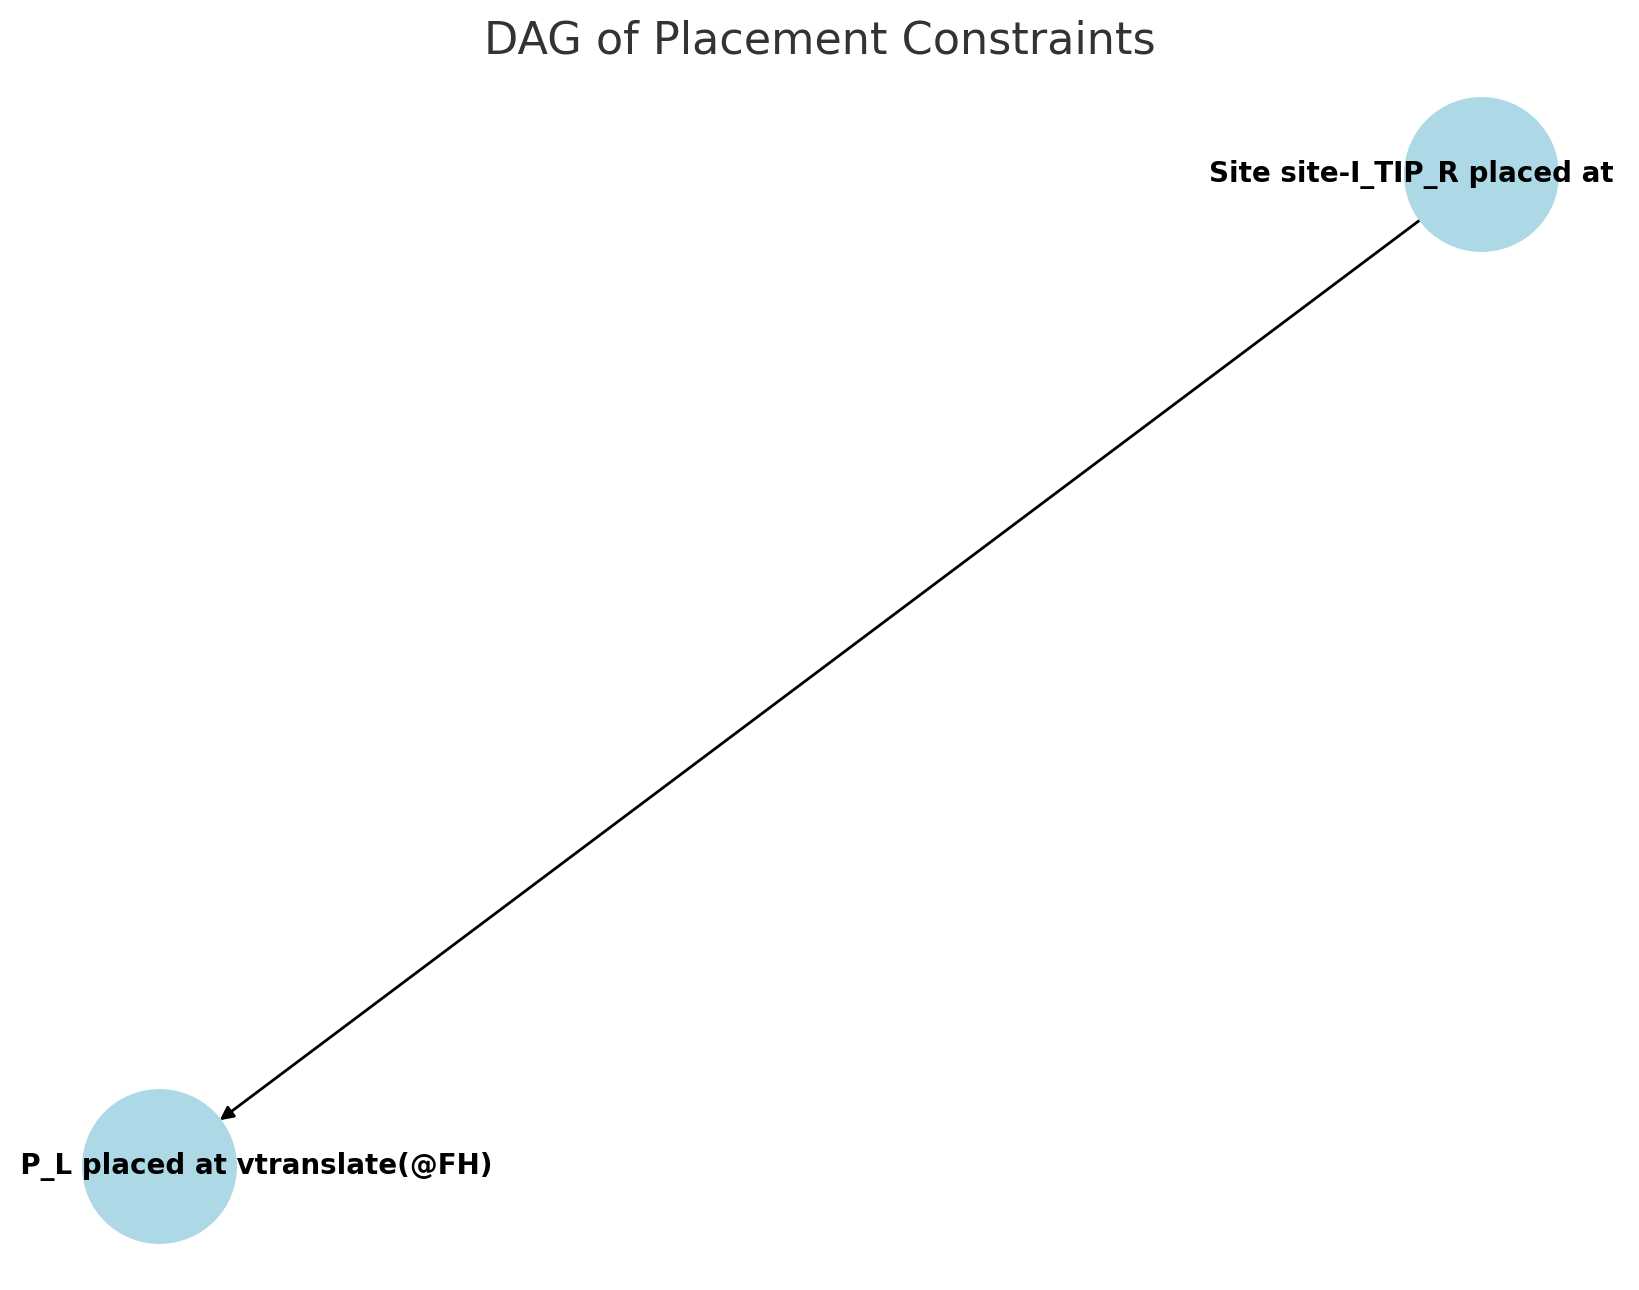
\includegraphics[width=0.8\textwidth]{chapters/multi_track/images/constraint_dag_cupboard.png}
    \caption{ConstraintDAG for a single block discource for the block HANDS\_CONTACT from the sign \emph{cupboard}.}
    \label{fig:constraint_dag_cupboard}
\end{figure}

\begin{figure}
    \centering
    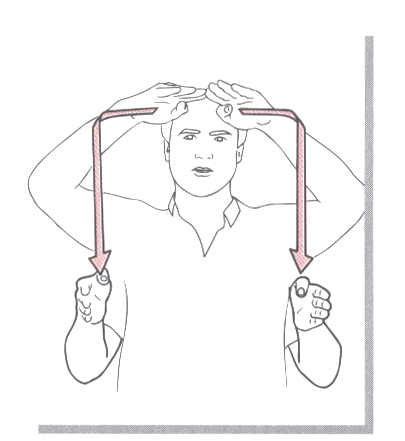
\includegraphics[width=0.8\textwidth]{chapters/multi_track/images/cupboard.jpg}
    \caption{Sign \emph{cupboard}~\cite{moody97}}
    \label{fig:cupboard}
\end{figure}

\subsection{Rule 1: Timely Evaluation}
\label{ch:multi_track:resolve_conflitcs:rule1}
\textbf{Problem:} Overlapping blocks with different start times.
\textbf{Solution:} Evaluate blocks chronologically to maintain logical sequence i.e. the block that starts first is evaluated first.
\textbf{Example:} Let's consider the timeline in figure~\ref{fig:azee_timeline} for the sign \emph{cupboard} (figure~\ref{fig:cupboard}). Here, blocks PALMS\_DOWN(palms facing down) and HANDS\_APART(hands being apart) overlap(effect the same bones i.e. the hand chains). Thus, the block that starts first, PALMS\_DOWN, is evaluated first. The HANDS\_APART block is evaluated after the PALMS\_DOWN block is finished.

\subsection{Rule 2: Constraint Precedence}
\label{ch:multi_track:resolve_conflitcs:rule2}
\textbf{Problem:} Order of topological sorting in case of 0 constraint dependencies for a block.
\textbf{Solution:} Follow the constraint precedence order: \emph{placement}, \emph{transpaths}, \emph{lookat}, \emph{trill}, \emph{orientation} and then \emph{morph}.
\textbf{Example:} Let's consider the same timeline in figure~\ref{fig:azee_timeline}. The block HANDS\_CONTACT optimizes placements first, then the orienations of the palm(coming from the block PALMS\_DOWN).

Non-overlapping blocks can be evaluated in parallel since they won't break the posture. Example, blocks PERM and HANDS\_CONTACT is non-overlapping block set in the sign \emph{armoire}.

\section{Second Pass}
\label{ch:multi_track:second_pass}

A second pass is done on the timeline to synthesize cyclic block sets, transpath, and hold blocks.

\subsection{Cyclic Block Set}
\label{ch:multi_track:second_pass:cyclic_blocks}

Cyclic block sets, as the name suggests, are blocks that effect each other cyclically. The figure~\ref{fig:cyclic_blocks} shows a cyclic block set for HANDS\_CONTACT and PALMS\_DOWN. This problem could arise if blocks effect a common heirarchy of the skeleton(any changes in parent will change the child even if the blocks don't effect that part of the skeleton). To deal with such sets, the blocks are evaluated again in a second pass by optimising for a \emph{cumulative flattened loss} i.e. cumulating loss of all constraints of the block set for the frame and optimising them together.

\begin{figure}[h]
    \centering
    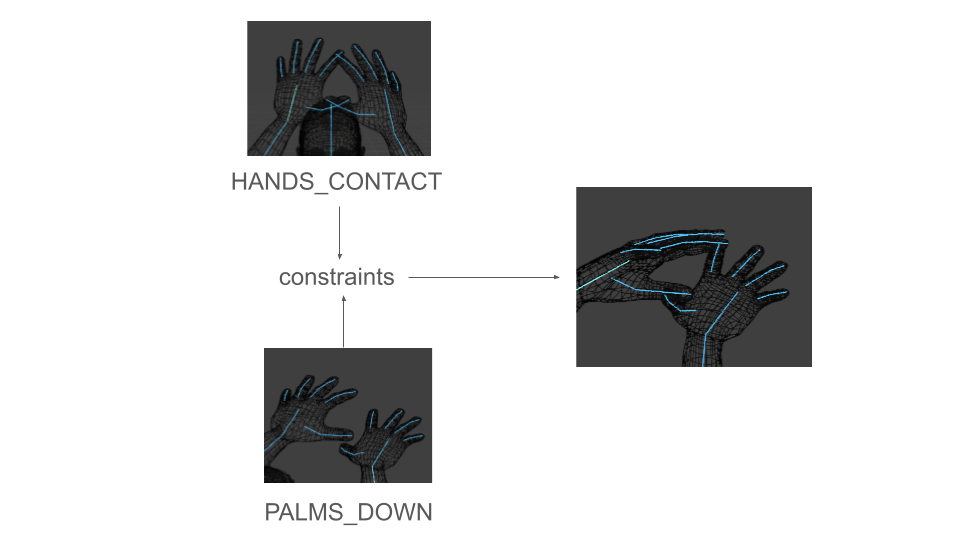
\includegraphics[width=0.8\textwidth]{chapters/multi_track/images/cyclic_blocks.png}
    \caption{Cyclic block set for PALMS\_DOWN and HANDS\_CONTACT}
    \label{fig:cyclic_blocks}
\end{figure}

\subsubsection{Baking Cyclic Blocks}
\label{ch:multi_track:second_pass:cyclic_blocks:baking_cyclic_blocks}

Even though the constraints are optimised together, each individual block in the cyclic block set is baked separately. This is done by collecting the \emph{change in motion curve} of each block and applying them separately to the skeleton after the optimization step (\ref{fig:baking_cyclic_blocks}).

\begin{figure}
    \centering
    \includegraphics[width=0.8\textwidth]{chapters/multi_track/images/baking_cyclic_blocks.png}
    \caption{Baking cyclic block sets}
    \label{fig:baking_cyclic_blocks}
\end{figure}

\subsection{Transpath Blocks}
\label{ch:multi_track:second_pass:transpath_blocks}

Transpath blocks are blocks which contain transpath constraints. A transpath constraint is a constraint that moves a body site along a path. It acts as an interpolation block but with a controlled path for a particular body site for it's preceding block and following blocks. The figure~\ref{fig:transpath_blocks} shows an example of transpath blocks for the sign \emph{cupboard}. Just like cyclic block sets, transpath blocks are evaluated in a second pass.

Transpath blocks are baked by evaluating the transpath constraint for each frame and applying the change in motion curve of the body site wrt to the preceding and the successing block. These motion curves are then baked as a new block.

\begin{figure}[h]
    \centering
    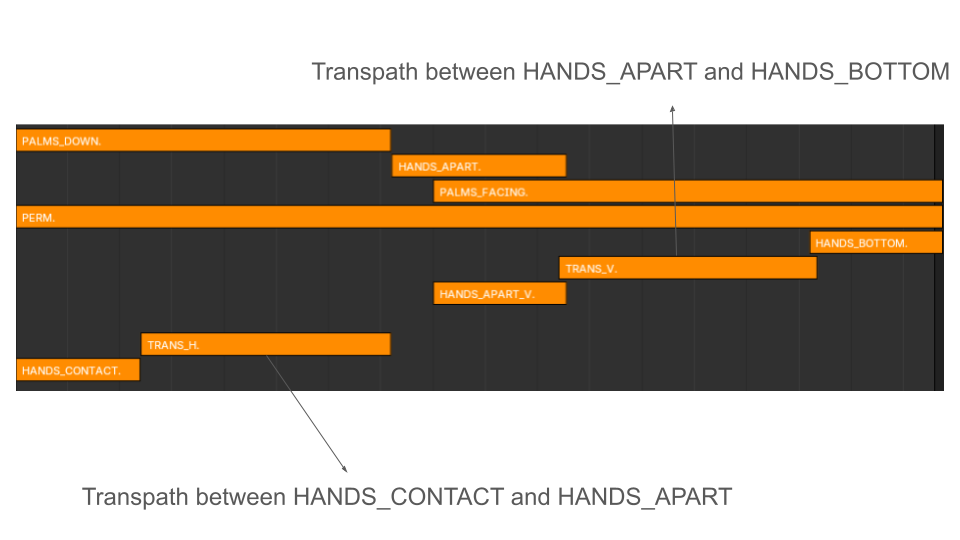
\includegraphics[width=0.8\textwidth]{chapters/multi_track/images/transpath_blocks.png}
    \caption{Transpath blocks in \emph{cupboard}}
    \label{fig:transpath_blocks}
\end{figure}

\subsection{Hold Blocks}
\label{ch:multi_track:second_pass:hold_blocks}

Hold blocks are blocks that hold another block for a certain duration. The figure~\ref{fig:hold_blocks} shows an example of hold blocks for the rule \emph{:info-about(:topic, :info)}. Hold blocks are also evaluated in the second pass since they hold another block(which has to be evaluated in the 1st pass).

Hold blocks are baked by extending the end of the motion curves of the block being held.

\begin{figure}
    \centering
    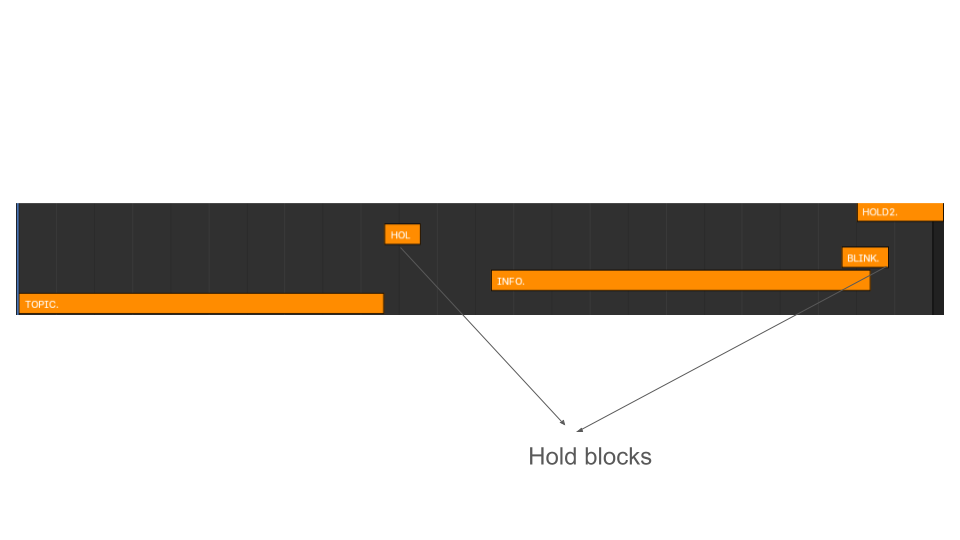
\includegraphics[width=0.8\textwidth]{chapters/multi_track/images/hold_blocks.png}
    \caption{Hold blocks for the rule \emph{:info-about(:topic, :info)}.}
    \label{fig:hold_blocks}
\end{figure}

\section{Pre-animated blocks}
\label{ch:multi_track:preanim_blocks}

The timeline can also contain pre-animated blocks. These blocks are blocks that contain pre-animated motion data. The pre-animated blocks are evaluated and baked first since they are independant of other blocks (figure~\ref{fig:preanim_blocks}).

\begin{figure}[h]
    \centering
    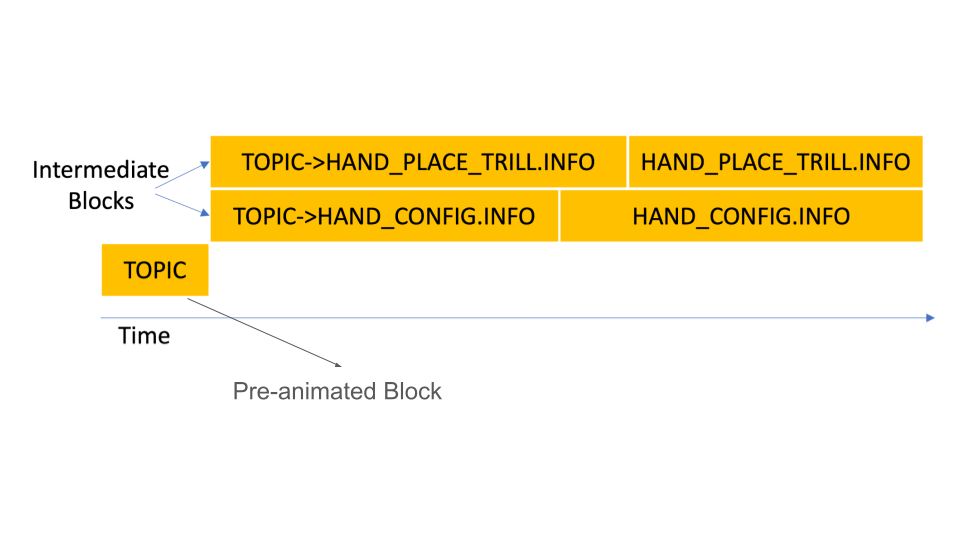
\includegraphics[width=0.8\textwidth]{chapters/multi_track/images/preanim_blocks.png}
    \caption{Pre-animated blocks in the multi-track timeline.}
    \label{fig:preanim_blocks}
\end{figure}

\section{Implementation and Results}
\label{ch:multi_track:implem_results}

The multi-track timeline is implementated in blender's non-linear editor. Each AZee Score, when animated, generates a blender action which is put on the non-linear editor as a strip with duration specified by the AZee \emph{sync rules}. The following table~\ref{tab:azee_to_blender} shows a non-exhaustive list of animated signs in blender with their corresponding generated timeline.

\begin{table}[h]
    \centering
    \begin{tabular}{|c|c|}
        \hline
        \textbf{Sign} & \textbf{Timeline} \\
        \hline
        \emph{tree} & figure todo \\
        \emph{cupboard} & figure todo \\
        \emph{...} & ... \\
        \hline
    \end{tabular}
    \caption{Animated signs in blender with their corresponding generated timeline.}
    \label{tab:azee_to_blender}
\end{table}

\section{Discussion}
\label{ch:multi_track:discussion}

The multi-track timeline approach to sign language synthesis offers several advantages over the existing existing method. Preserving the multi-track information and dynamics present in the AZee description provides us the stepping stones to integrate pre-animated motion data which was not possible with the previous low-level AZee synthesizor. The non-linear synthesis allows for the correct execution order of blocks and avoids conflicts. On top of that, hybrid constucts such as \emph{dynamic points} (a point changing it's location over time) can be easily integrated into the timeline (figure~\ref{fig:dynpoint_example}).

\begin{figure}[h]
    \centering
    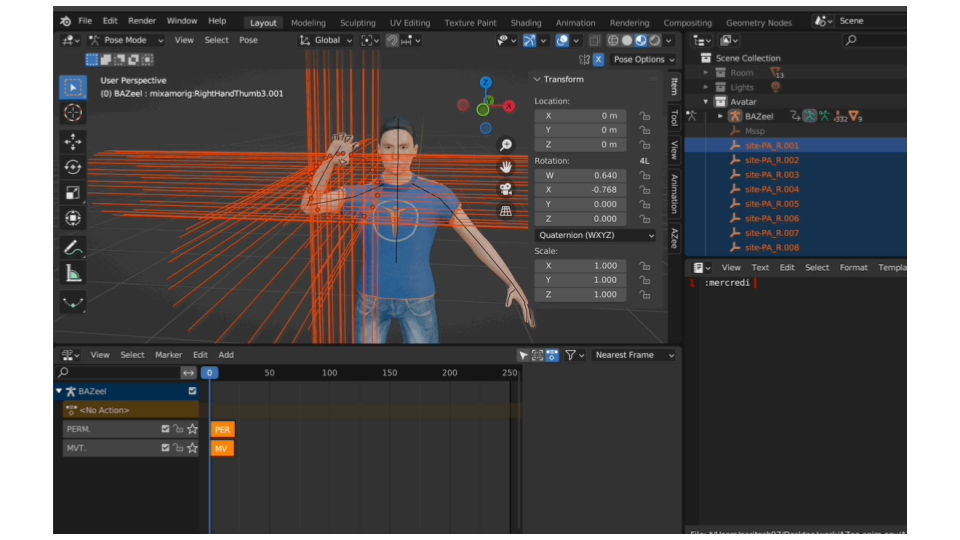
\includegraphics[width=0.8\textwidth]{chapters/multi_track/images/dynpoint_example.png}
    \caption{Example of a dynamic point in the multi-track timeline.}
    \label{fig:dynpoint_example}
\end{figure}

\end{document}
